\documentclass{beamer}
%\usepackage{geometry}
%\geometry{paperwidth=1920mm,paperheight=1000mm}
\usepackage[orientation=landscape,size=a0,scale=1.3,debug]{beamerposter}
%width=192,height=108,scale=1.4
\mode<presentation>{\usetheme{RWTH2}}
\usepackage{chemformula}
\usepackage[utf8]{inputenc}
\usepackage[german, english]{babel} % required for rendering German special characters
\usepackage{siunitx} %pretty measurement unit rendering
\usepackage{hyperref} %enable hyperlink for urls
\usepackage{ragged2e}
\usepackage[font=scriptsize,justification=justified]{caption}
\usepackage{array,booktabs,tabularx}
\usepackage[autostyle=true,german=quotes,english=american]{csquotes}

\usepackage{amsmath, mhchem} % Unterstützung für mathematische und chemische Formeln

\usepackage{floatflt}

\usepackage[authoryear]{natbib}
\bibliographystyle{apalike}

\newcolumntype{Z}{>{\centering\arraybackslash}X} % centered tabularx columns
\sisetup{per=frac,fraction=sfrac}

\title{Bayesian Decision Theory in Structural Geological Modeling - \\ How
Reducing Uncertainties Affects Reservoir Value Estimations}
%\author{Fabian Antonio Stamm$^{1}$}
%\institute[RWTH Aachen University]{$^{1}$Institute of Computational Geoscience and Reservoir Engineering, RWTH Aachen University, Germany}
\author{Fabian Antonio Stamm, Miguel de la Varga, Alexander Schaaf, Florian Wellmann}
%\author{Fabian Antonio Stamm$^{1}$, Miguel de la Varga$^{1}$, Alexander Schaaf$^{1}$, Florian Wellmann$^{1}$}
\institute[RWTH Aachen University]{Institute of Computational Geoscience and Reservoir Engineering, RWTH Aachen University, Germany}
\date{\today}

% edit this depending on how tall your header is. We should make this scaling automatic :-/
\newlength{\columnheight}
\setlength{\columnheight}{104cm}

\begin{document}
\begin{frame}

\begin{columns}

	\begin{column}{.249\textwidth}
		\begin{beamercolorbox}[center]{postercolumn}
			\begin{minipage}{.98\textwidth}  % tweaks the width, makes a new \textwidth
				\parbox[t][\columnheight]{\textwidth}{ % must be some better way to set the the height, width and textwidth simultaneously				
				
				
\begin{myblock}{1 - Introduction}
Structural geological modeling is of central importance for the assessment of uncertain hydrocarbon accumulations in potential reservoirs. Hydrocarbon exploration and production is a high-risk, high-reward sector in which good decision making is indispensable.
Utilizing a Bayesian approach, we examine the influence of model uncertainties and respective uncertainty changes on the decision making of actors in this field.
%Actors in this field are faced with numerous uncertainties that have to be considered. We examine respective decision making from a Bayesian perspective. 
%...building on recent developments that have transferred this probabilistic approach to address uncertainties in the field of structural geological modeling.
%We examine respective decision making from a Bayesian perspective by considering two main approaches: (1) we treat geological modeling as a Bayesian inference problem, so that additional geological information can be incorporated as likelihood functions linked to prior parameters in a probabilistic framework; (2) we base the decision-making step on value estimation by optimizing a case-specific loss function.

\end{myblock}					
					
\begin{myblock}{2 - Methods}
\textbf{Construction of a 3D structural geological model:}
	\begin{itemize}
	%\item Model creation using GemPy (see \citet{gmd-2018-61})
	\item Synthetic model of a simple anticline-fault trap in a potential hydrocarbon system (see Figure \ref{fig:unc_lik})
	\item Inclusion of uncertainties by assigning probability distributions to the positions of layer interfaces in depth
	\end{itemize}							
								\vspace{0.5em}
								\begin{figure}
									\begin{minipage}{0.95\textwidth}
										\centering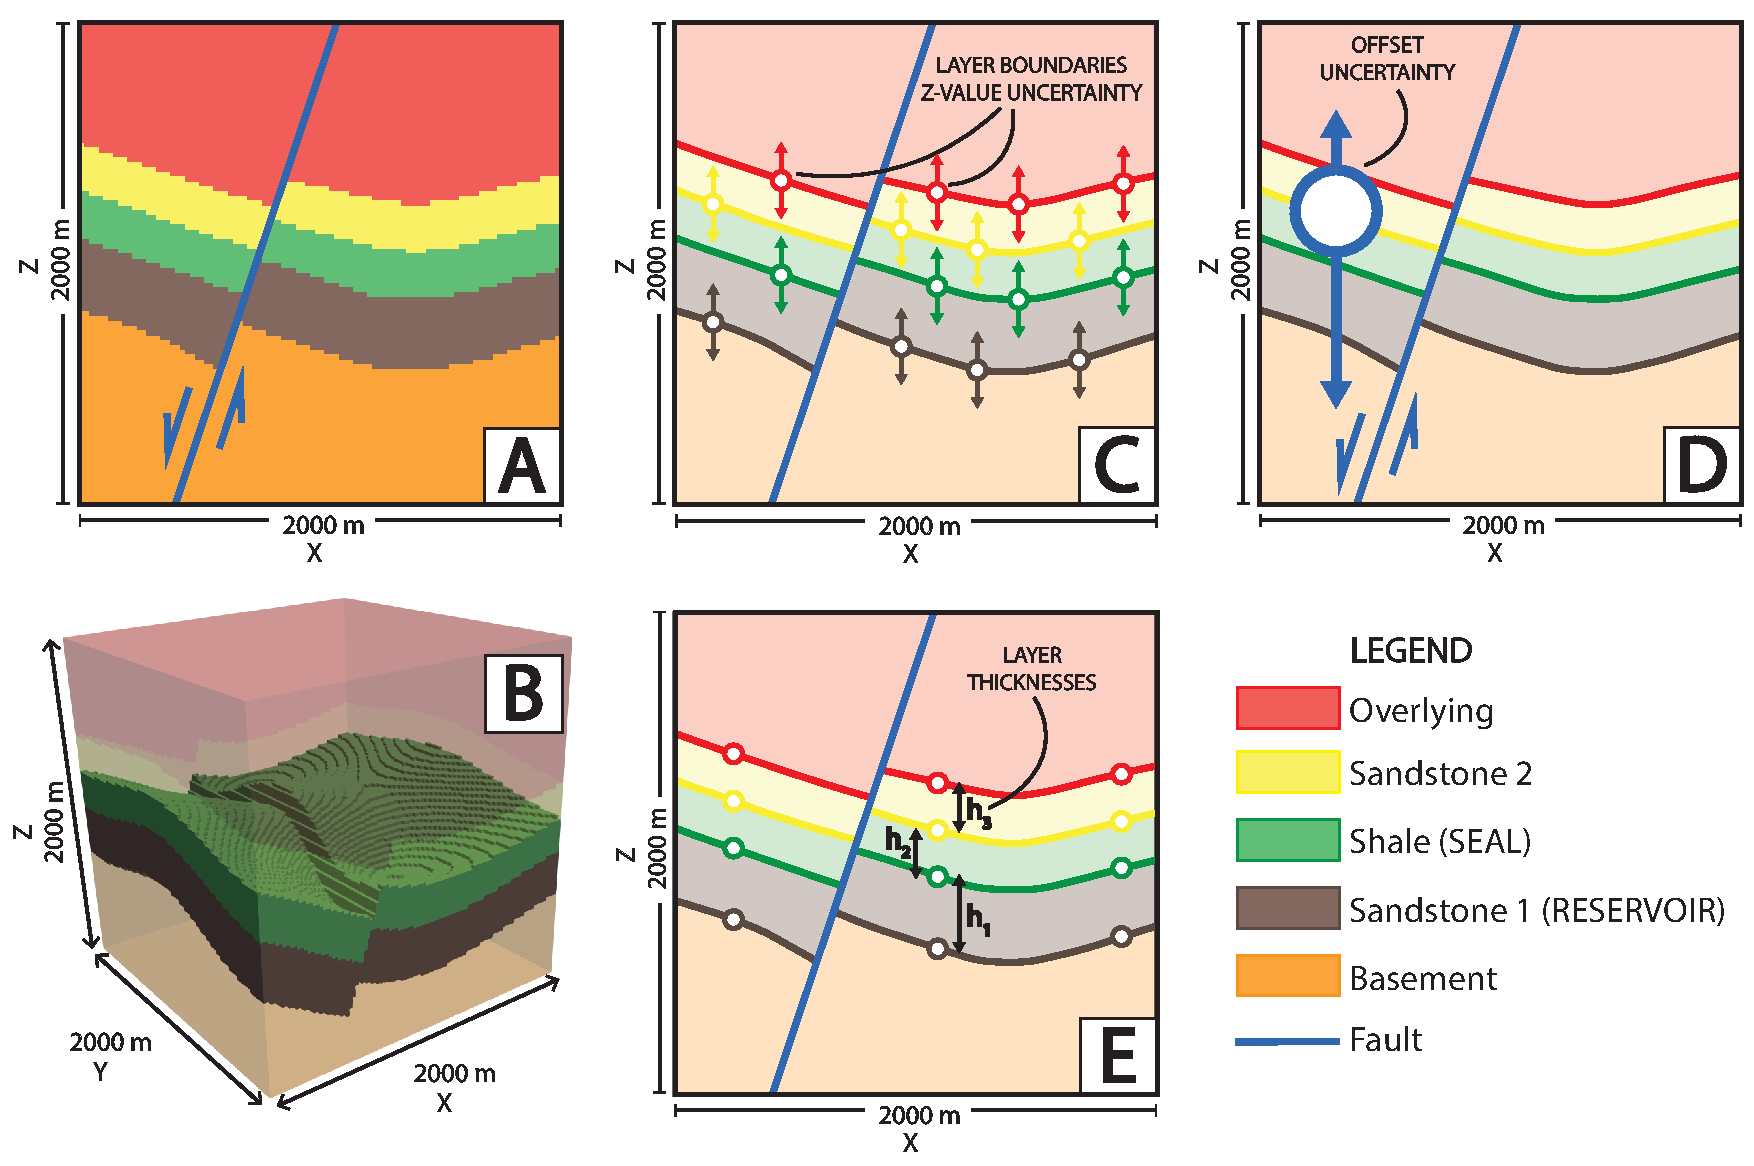
\includegraphics[width=1\textwidth]{figures/Uncertainties_Likelihoods.pdf}
										\caption{The structural geological model illustrated as a 2D cross section (A) and a 3D voxel representation (B). The inclusion of $z$-positional uncertainties affecting layer depths and fault offset are depicted in (C) and (D). Thicknesses of the three middle layers are defined by the distances of interface points (E) and are thus directly dependent on (C).}
										\label{fig:unc_lik}
									\end{minipage}
								\end{figure}
\textbf{Integration in a probabilistic modeling framework for Bayesian analysis:}
	\begin{itemize}
	%\item Utilizing PyMC (see \citet{salvatier2016pymc3})
	\item Setting up a full probability model taking into account all parameter probability distributions
	\item Bayesian inference: Conditioning of parameters on additionally observed data via likelihood functions
	\item Approximation of posterior distributions through the use of MCMC sampling
	\end{itemize}
\textbf{Evaluation of modeling results:}
										\begin{itemize}
										\item Shannon entropy for uncertainty visualization (after \citet{wellmann2012uncertainties})
										\item Implementation of customized algorithms for structural analysis, trap recognition (see Figure \ref{fig:trap_cond}) and calculation of recoverable oil volumes (ROV)
										\item Decision making based on the optimization of a case-specific loss function that is employed to estimate the ROV as the crucial reservoir value %that considers differently risk-affine actors
										\end{itemize}
										
	\vspace{0.1em}
						
\end{myblock}\vfill
					
					
		}\end{minipage}\end{beamercolorbox}
	\end{column}



\begin{column}{.499\textwidth}
	\begin{beamercolorbox}[center]{postercolumn}
		\begin{minipage}{.98\textwidth} % tweaks the width, makes a new \textwidth
				\parbox[t][\columnheight]{\textwidth}{ % must be some better way to set the the height, width and textwidth simultaneously					
					
\begin{myblock}{2 - Methods (continued)}
\vspace{0.5em}
%\textbf{Evaluation of modeling results:}
%	\begin{itemize}
%	\item Shannon entropy for uncertainty visualization (after \citet{wellmann2012uncertainties}.
%	\item Implementation of algorithms for structural analysis, trap recognition (see Figure \ref{fig:trap_cond}) and calculation of recoverable oil volumes (ROV)
%	\item Decision making based on the optimization of a case-specific custom loss function that considers differently risk-affine actors
%	\end{itemize}
	
	%We examine respective decision making from a Bayesian perspective by considering two main
	%approaches: (1) we treat geological modeling as a Bayesian inference problem, so that additional geological
	%information can be incorporated as likelihood functions linked to prior parameters in a probabilistic framework; (2)
	%we base the decision-making step on value estimation by optimizing a case-specific loss function. This function is
	%customized to reflect the decision making of differently risk-affine actors relative to previously computed reservoir
	%value probability distributions.
	%We apply our approach to synthetic geological models which are constructed to represent potential hydro-
	%carbon systems. Markov chain Monte Carlo sampling is used to approximate posterior models of reduced
	%uncertainty. 	

	%For the valuation of prior and posterior models, we also develop algorithms for automatic trap
	%	recognition and volume calculation.	
							
								\begin{minipage}[h]{0.6\textwidth} %0.656
								\textbf{Custom loss function design:}
								
								We regard decision making as the process of estimating the posterior ROV by optimizing a customized loss function that considers the preferences of differently risk-affine actors. A decision that minimizes expected loss, according to such a function, is referred to as Bayes action \citep{davidson2015}. We extend the standard absolute-error loss function with a risk factor \textit{r} and several other weighting factors to express the expected loss relative to the nature and magnitude of deviation of the estimate $\hat{\theta}$ from the true value $\theta$:								
								
								\begin{equation*} %\label{eq:LFR_final}
																L(\theta,\hat{\theta}) =
																\begin{cases}
																|\theta - \hat{\theta}|*r^{-0.5}, & \text{for } 0<\hat{\theta}<\theta  \\
																|\theta-\hat{\theta}|*a*r, & \text{for } 0<\theta<\hat{\theta} \\
																|\theta-\hat{\theta}|*b*r, & \text{for } \theta\leq0<\hat{\theta} \\
																|\theta-\hat{\theta}|*c*r^{-0.5}, & \text{for } \hat{\theta}\leq0<\theta 
																\end{cases},
																\text{ with } a,b,c,r \in \mathbb{Q}.
								\end{equation*}
								
								We define that normal overestimation is 25\% (\textit{a} = 1.25), fatal overestimation 100\% (\textit{b} = 2) and fatal underestimation 50\% (\textit{c} = 1.5) worse than normal underestimation. A risk factor \textit{r} = 1 represents risk neutrality, while \textit{r} $<$ 1 expresses risk-friendly, and \textit{r} $>$ 1 risk-averse behavior.
								
								\end{minipage}\hspace{0.005\textwidth}
								%\vspace{0.5em}
								\begin{minipage}{0.39\textwidth}
								\begin{figure}
									\centering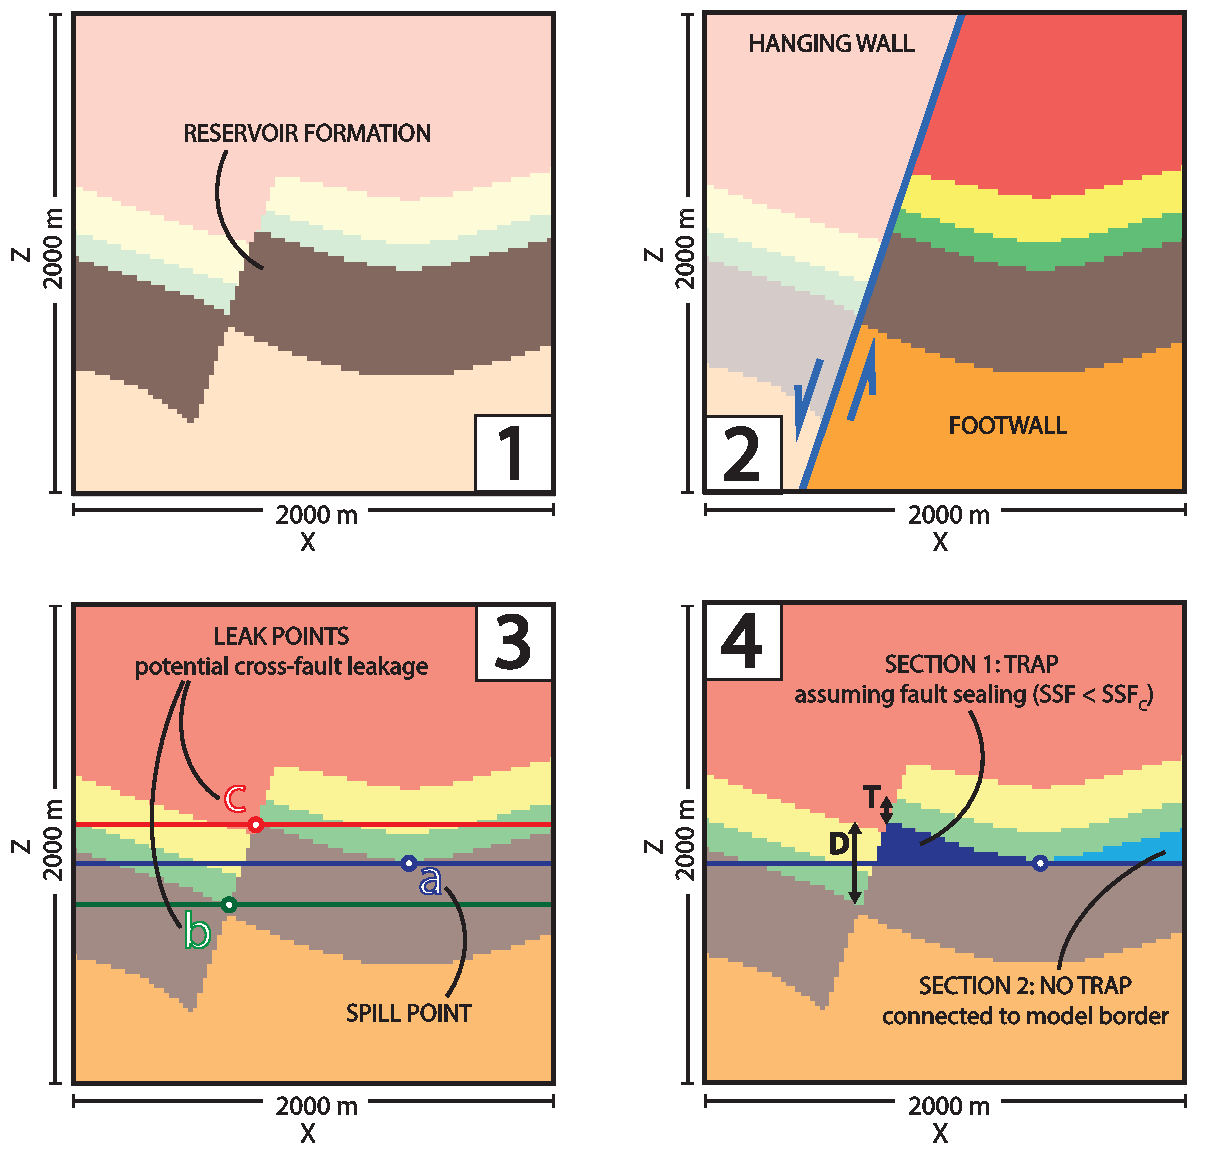
\includegraphics[width=1\textwidth]{figures/Trap_Cond_H.pdf}
									\caption{To be recognized as part of a trap, a reservoir voxel (1) has
									to be positioned in the	footwall (2). The maximum trap fill is defined by either the anticlinal spill point (3;a) or a point of leakage across the fault, depending on juxtapositions with layers
									underlying (3;b) or overlying the seal (3;c). The latter is only relevant if the
									critical Shale Smear Factor (SSF$_c$) is exceeded, as determined over D and T in (4). Voxels connected to the model border are discarded.}
									\label{fig:trap_cond}
									%Trap closure is defined by the seal shape and the normal fault (3).
								\end{figure}
								%\begin{figure}
								%	\centering
								%	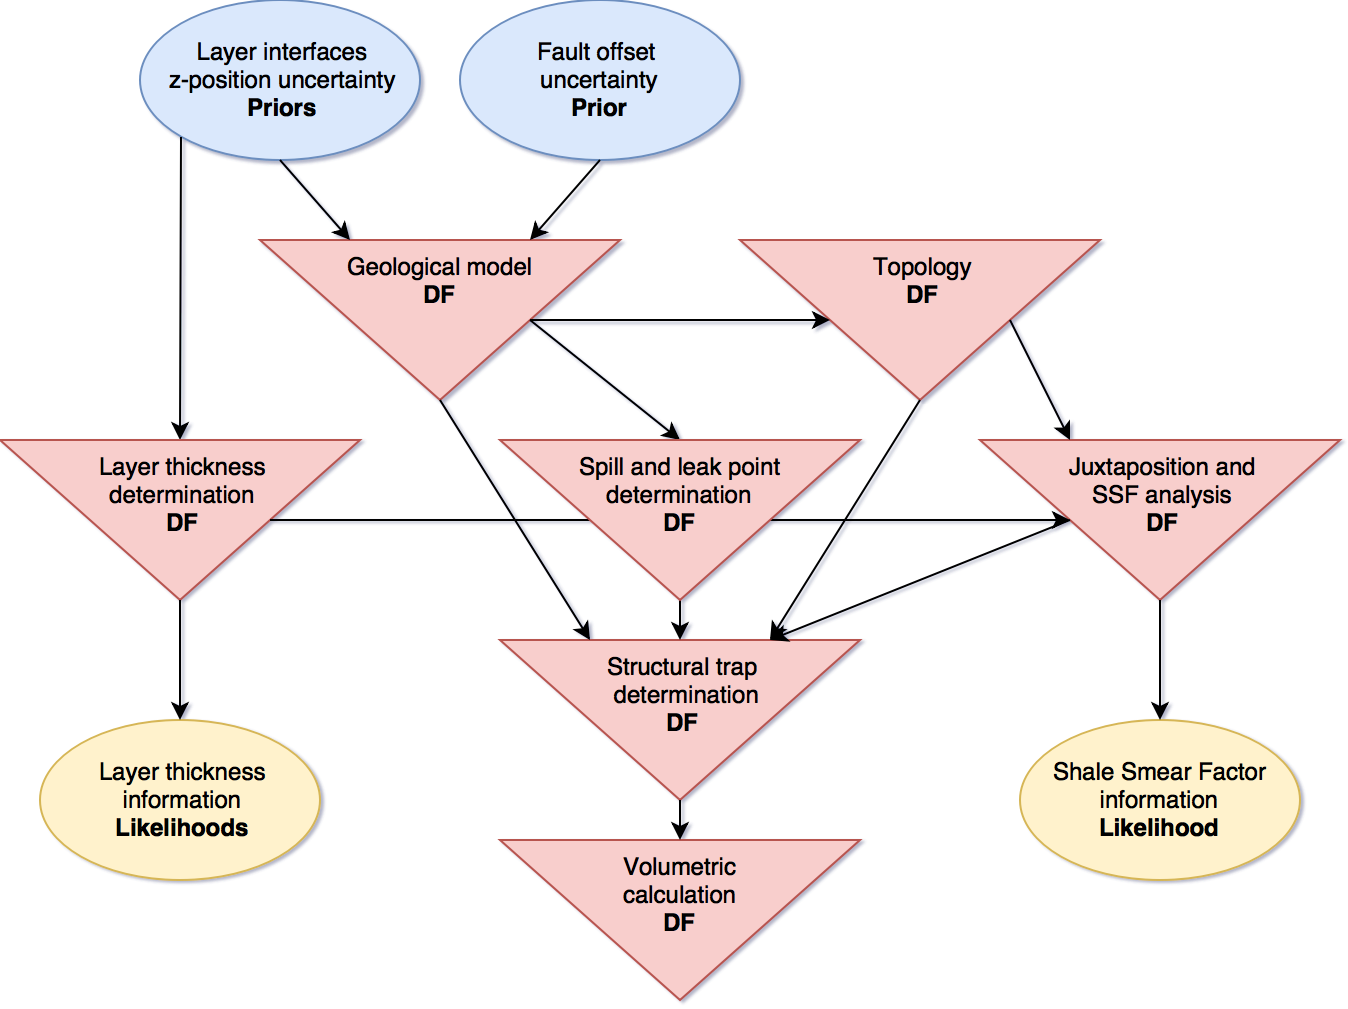
\includegraphics[width=1\textwidth]{figures/model_network}
								%	\caption{Illustration of the probabilistic model as a hierarchical Bayesian network after \citet{koller2009probabilistic}. Stochastic nodes are represented by ellipses (blue for
								%	priors, yellow for likelihoods). Deterministic functions are depicted as triangles in
								%	red. Arrows indicate direct connections from parent to child nodes.}
								%	\label{fig:model_network}
								%\end{figure}
								\end{minipage}
								%\begin{minipage}{0.327\textwidth}
								
								%\end{minipage}
\end{myblock}
								
\begin{myblock}{3 - Results}				
	\vspace{0.1em}
	\begin{figure}
		\begin{minipage}{0.99\textwidth}
			%\hfill
			\begin{minipage}[t]{0.49\textwidth}
				\centering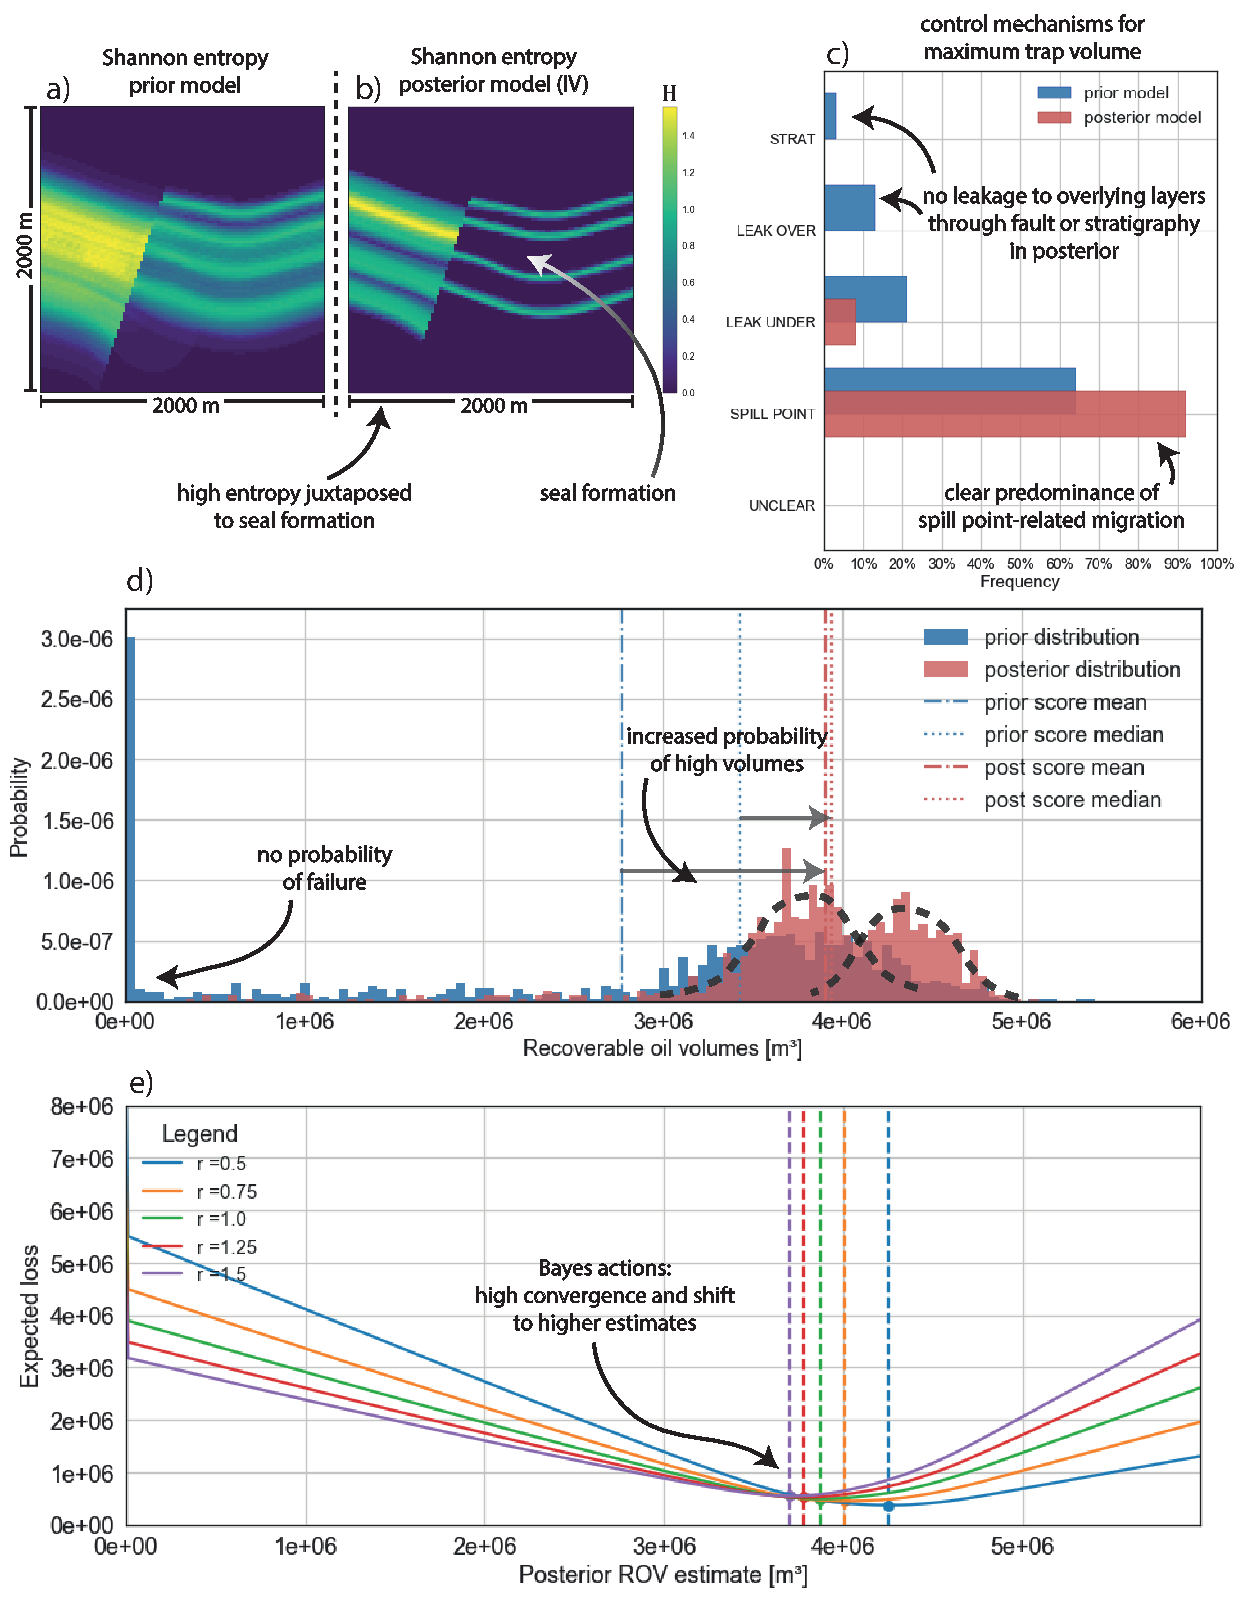
\includegraphics[width=1\textwidth]{figures/ML4.pdf}
				\caption{Evaluation of a model conditioned on thickness and SSF likelihoods which assure a reliable trap closure and reinforce the probability of a high ROV. Shannon entropy is significantly reduced in the posterior model (b). Cross-fault leakage to overlying layers is eliminated as a trap control mechanism (c) and coincides with the disappearance of the probability of failure in the posterior ROV distribution (d). The respective loss functions are plotted in (e), showing high decision convergence.}
				%\caption{Evaluation of a model conditioned on thickness and SSF likelihoods which reinforce the probability of a high ROV and a reliable trap closure.}
				%\caption{Evaluation of a model conditioned on thickness and SSF likelihoods which assure a reliable trap closure and reinforce the probability of a high ROV. Shannon entropy was significantly reduced in the posterior model (b). Cross-fault leakage to overlying layers was eliminated as a trap control mechanism (c) and coincides with the disappearance of the probability of failure in the posterior ROV distribution (d). The respective loss functions are plotted in (e), showing high decision convergence.}
				\label{fig:ML4}
			\end{minipage}\hfill
			%\hspace{length=0.1\textwidth}
			\begin{minipage}[t]{0.49\textwidth}
				\centering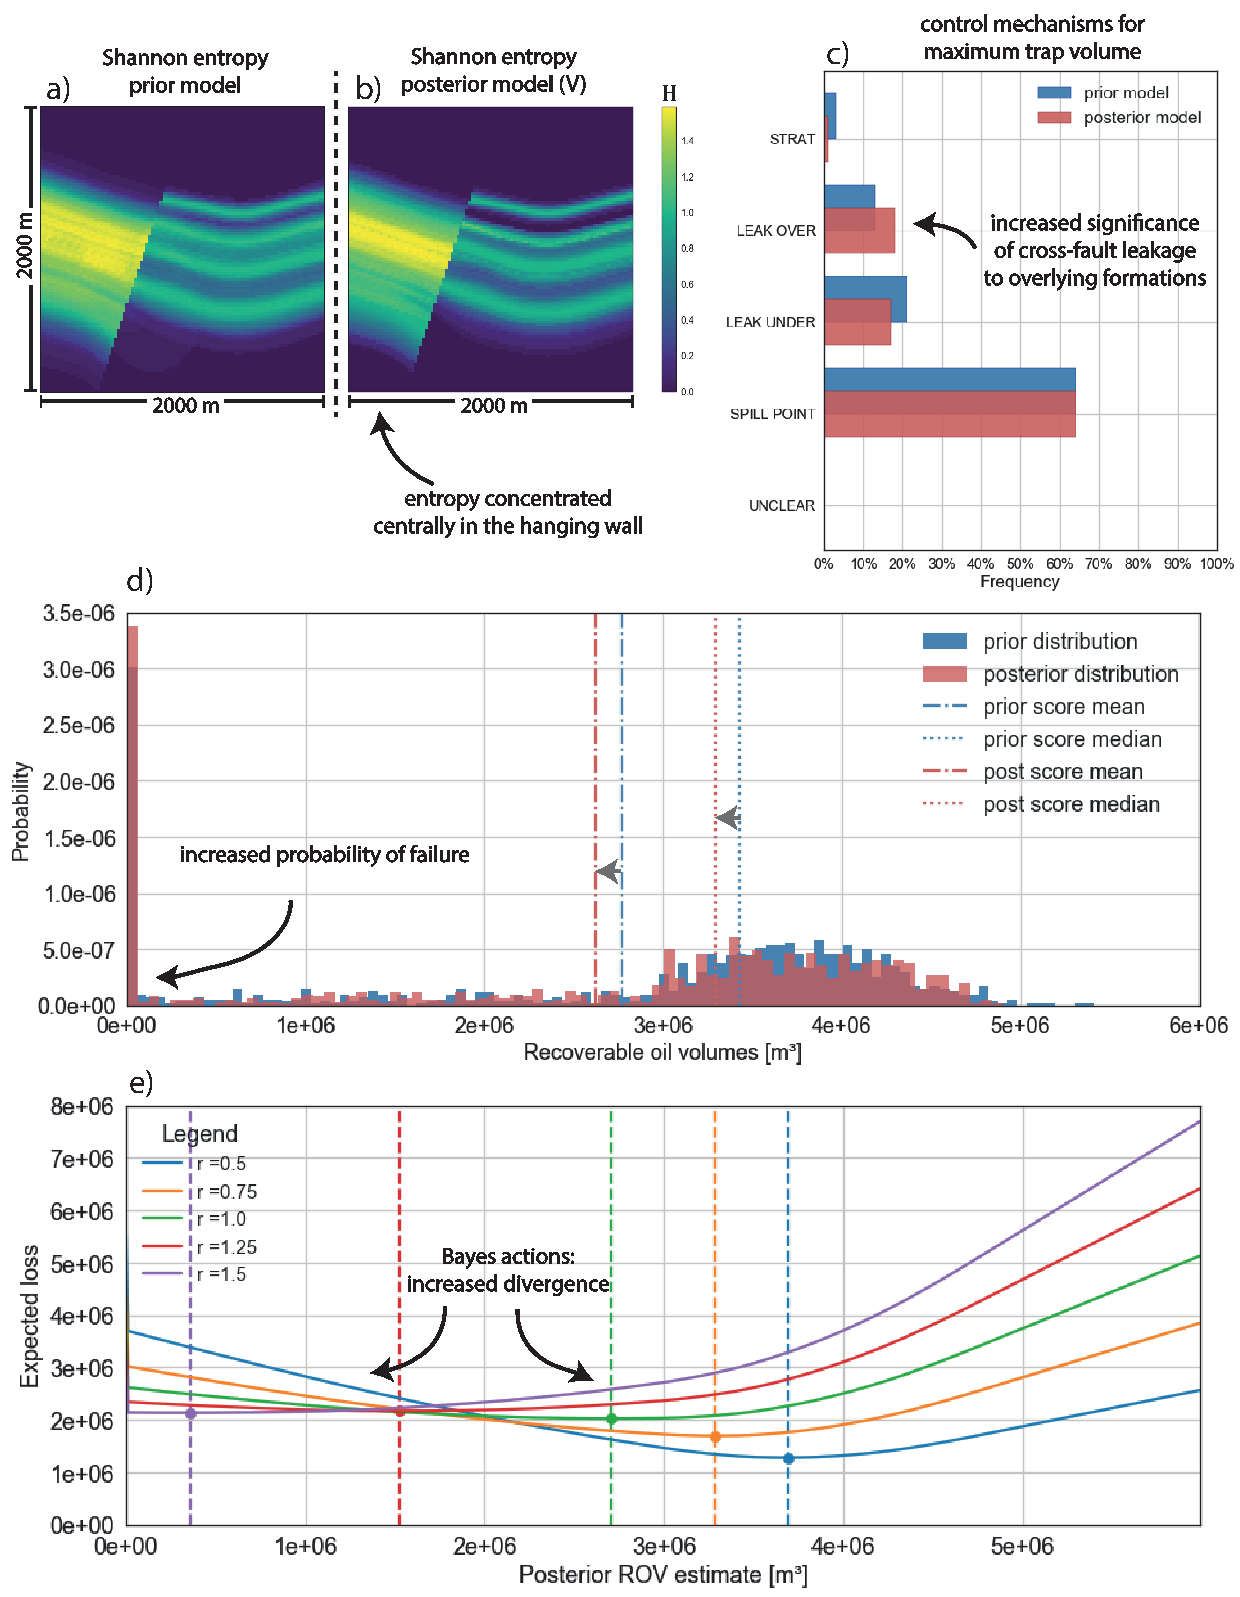
\includegraphics[width=1\textwidth]{figures/ML5.pdf}
				\caption{Evaluation of a model conditioned on a SSF likelihood which narrows around the critical SSF$_c$ and thus amplifies the duality in the posterior ROV distribution (d). Shannon entropy is only slightly diminished (a,b). general cross-fault leakage remains a significant trap control mechanism (c). The resulting loss function realizations show a high divergence of differently risk-affine decisions.}
				%\caption{Evaluation of a model conditioned on a SSF likelihood which narrows around the critical SSF$_c$ and thus amplifies the duality in the posterior ROV distribution (d).}
				\label{fig:ML5}
			\end{minipage}	
			%\hfill
		\end{minipage}
	\end{figure}

%	\vspace{0.5em}
%	\begin{figure}
%		\begin{minipage}{0.95\textwidth}
%			\begin{minipage}[t]{0.32\textwidth}
%				\centering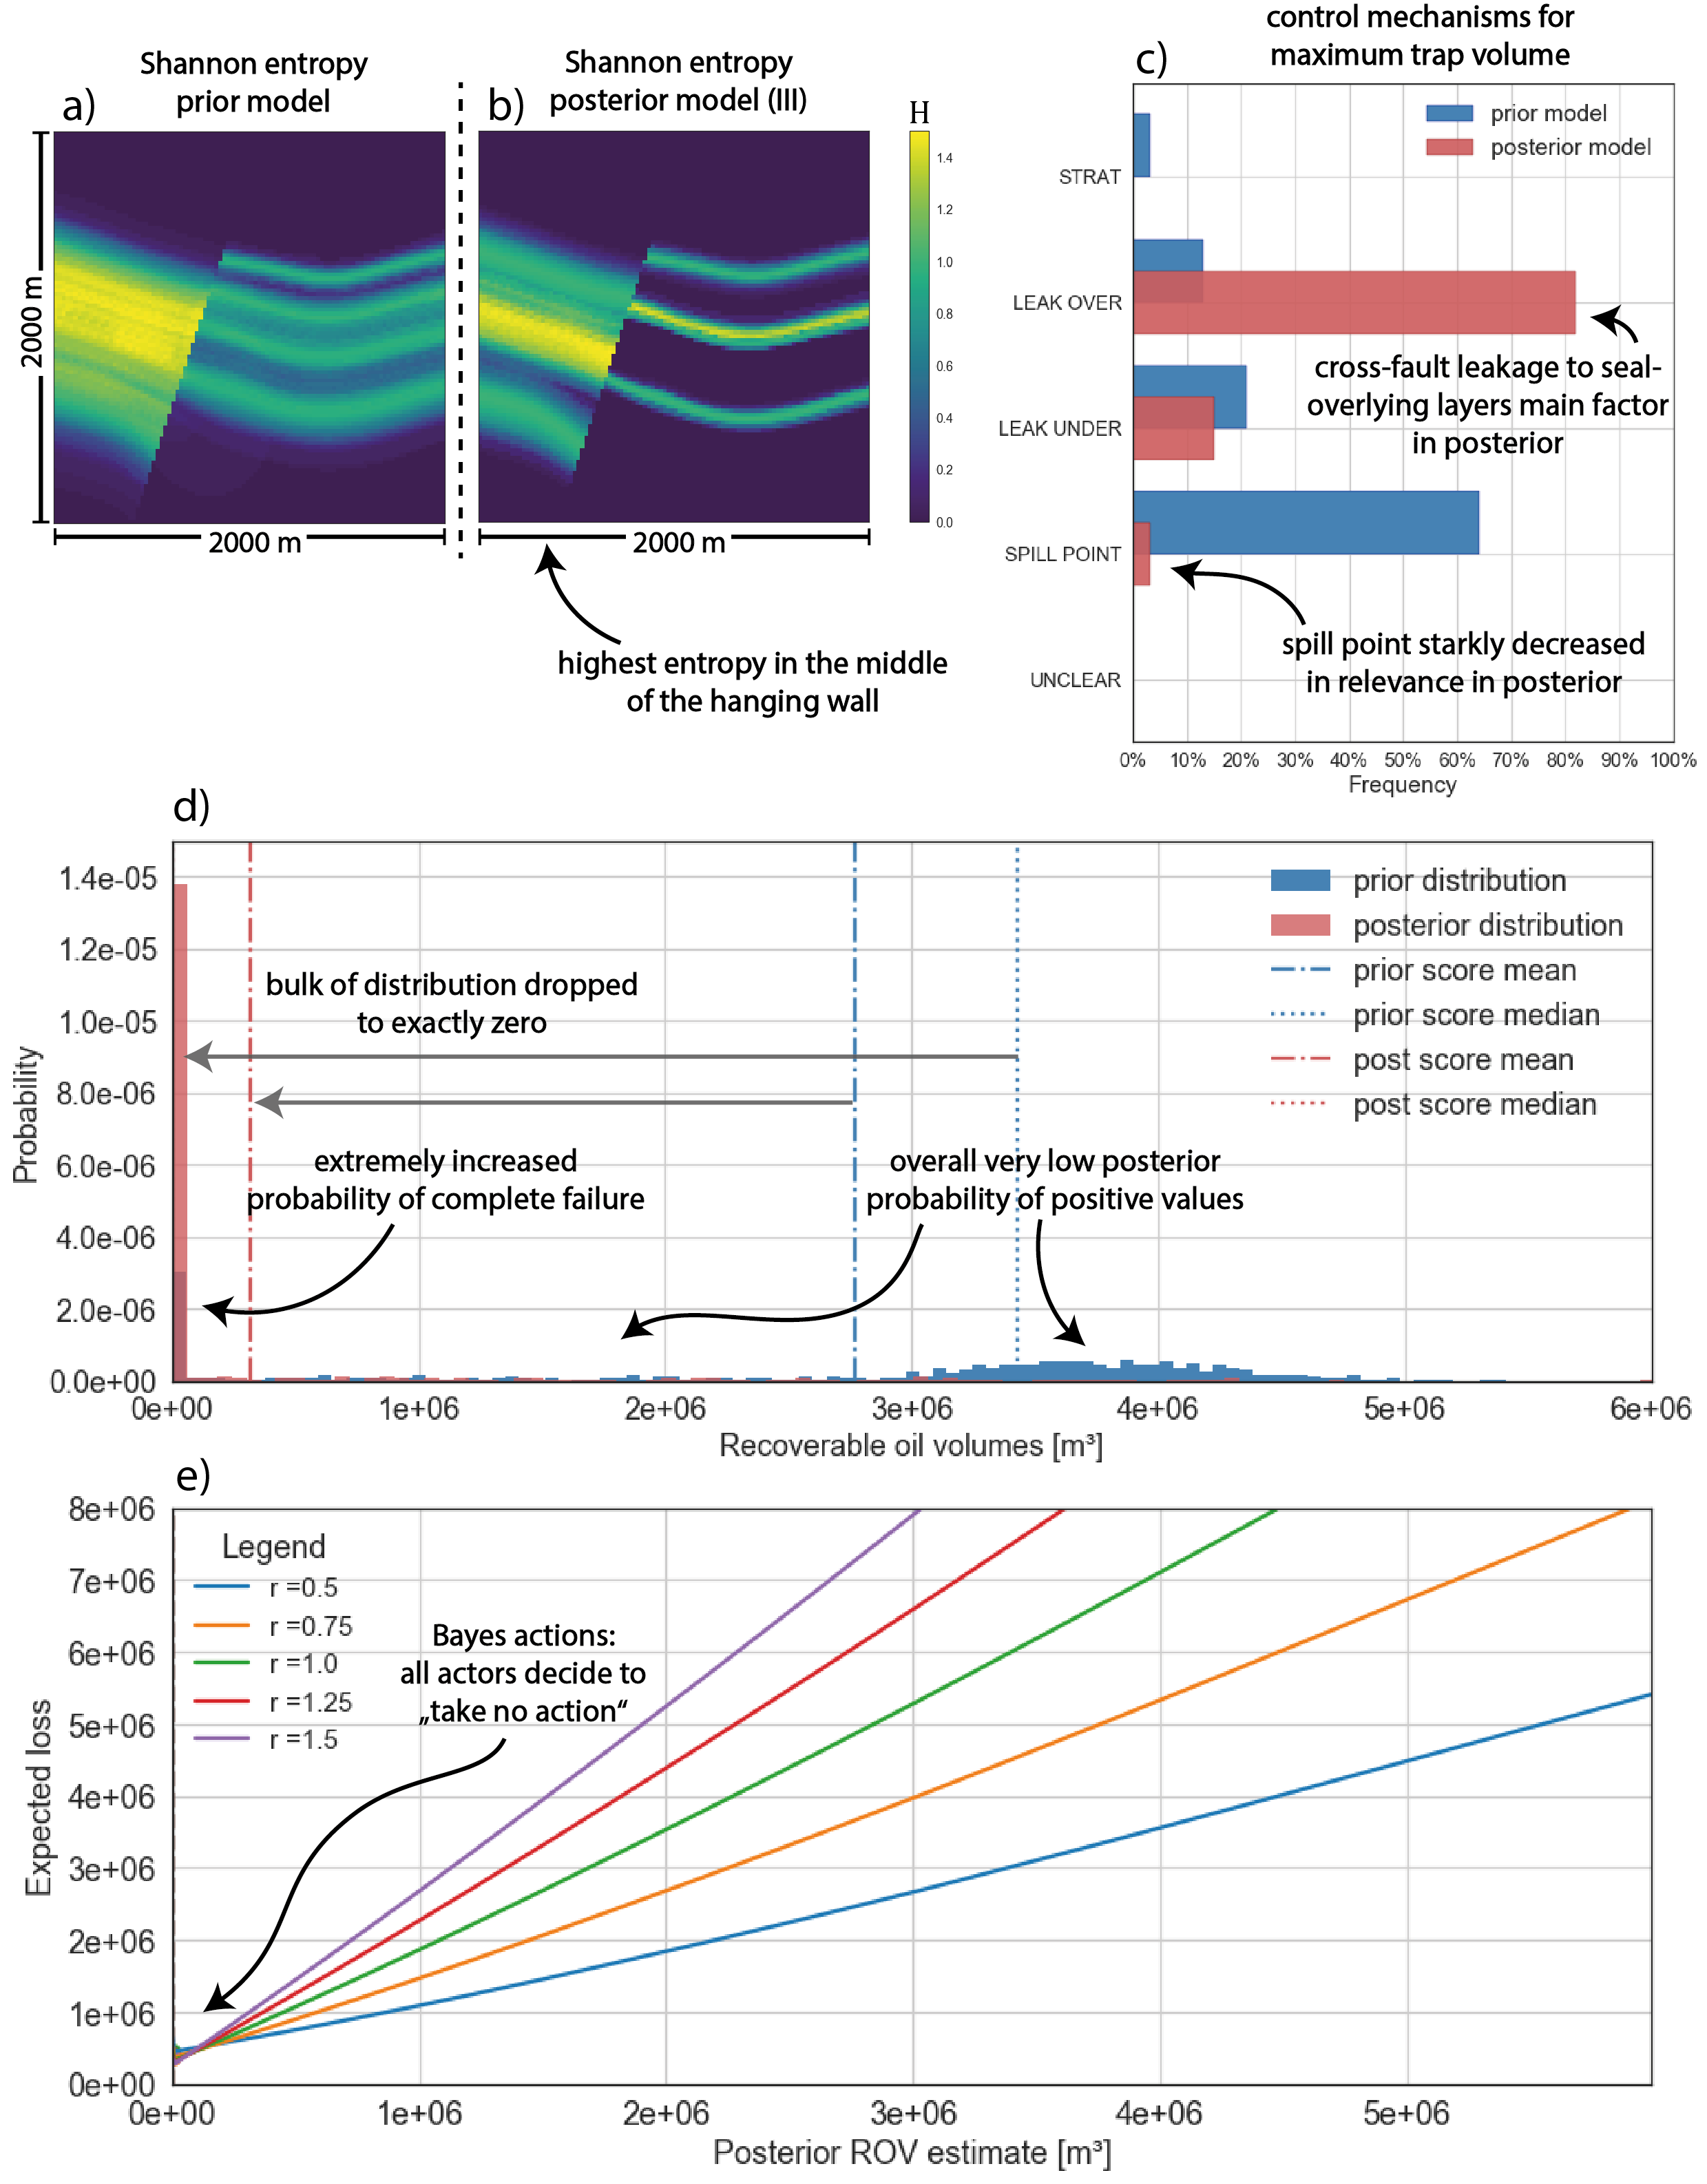
\includegraphics[width=1\textwidth]{figures/ML2}
%				\caption{...}
%				\label{fig:ML2}
%			\end{minipage}
%			\hspace{\fill}
%			\begin{minipage}[t]{0.32\textwidth}
%				\centering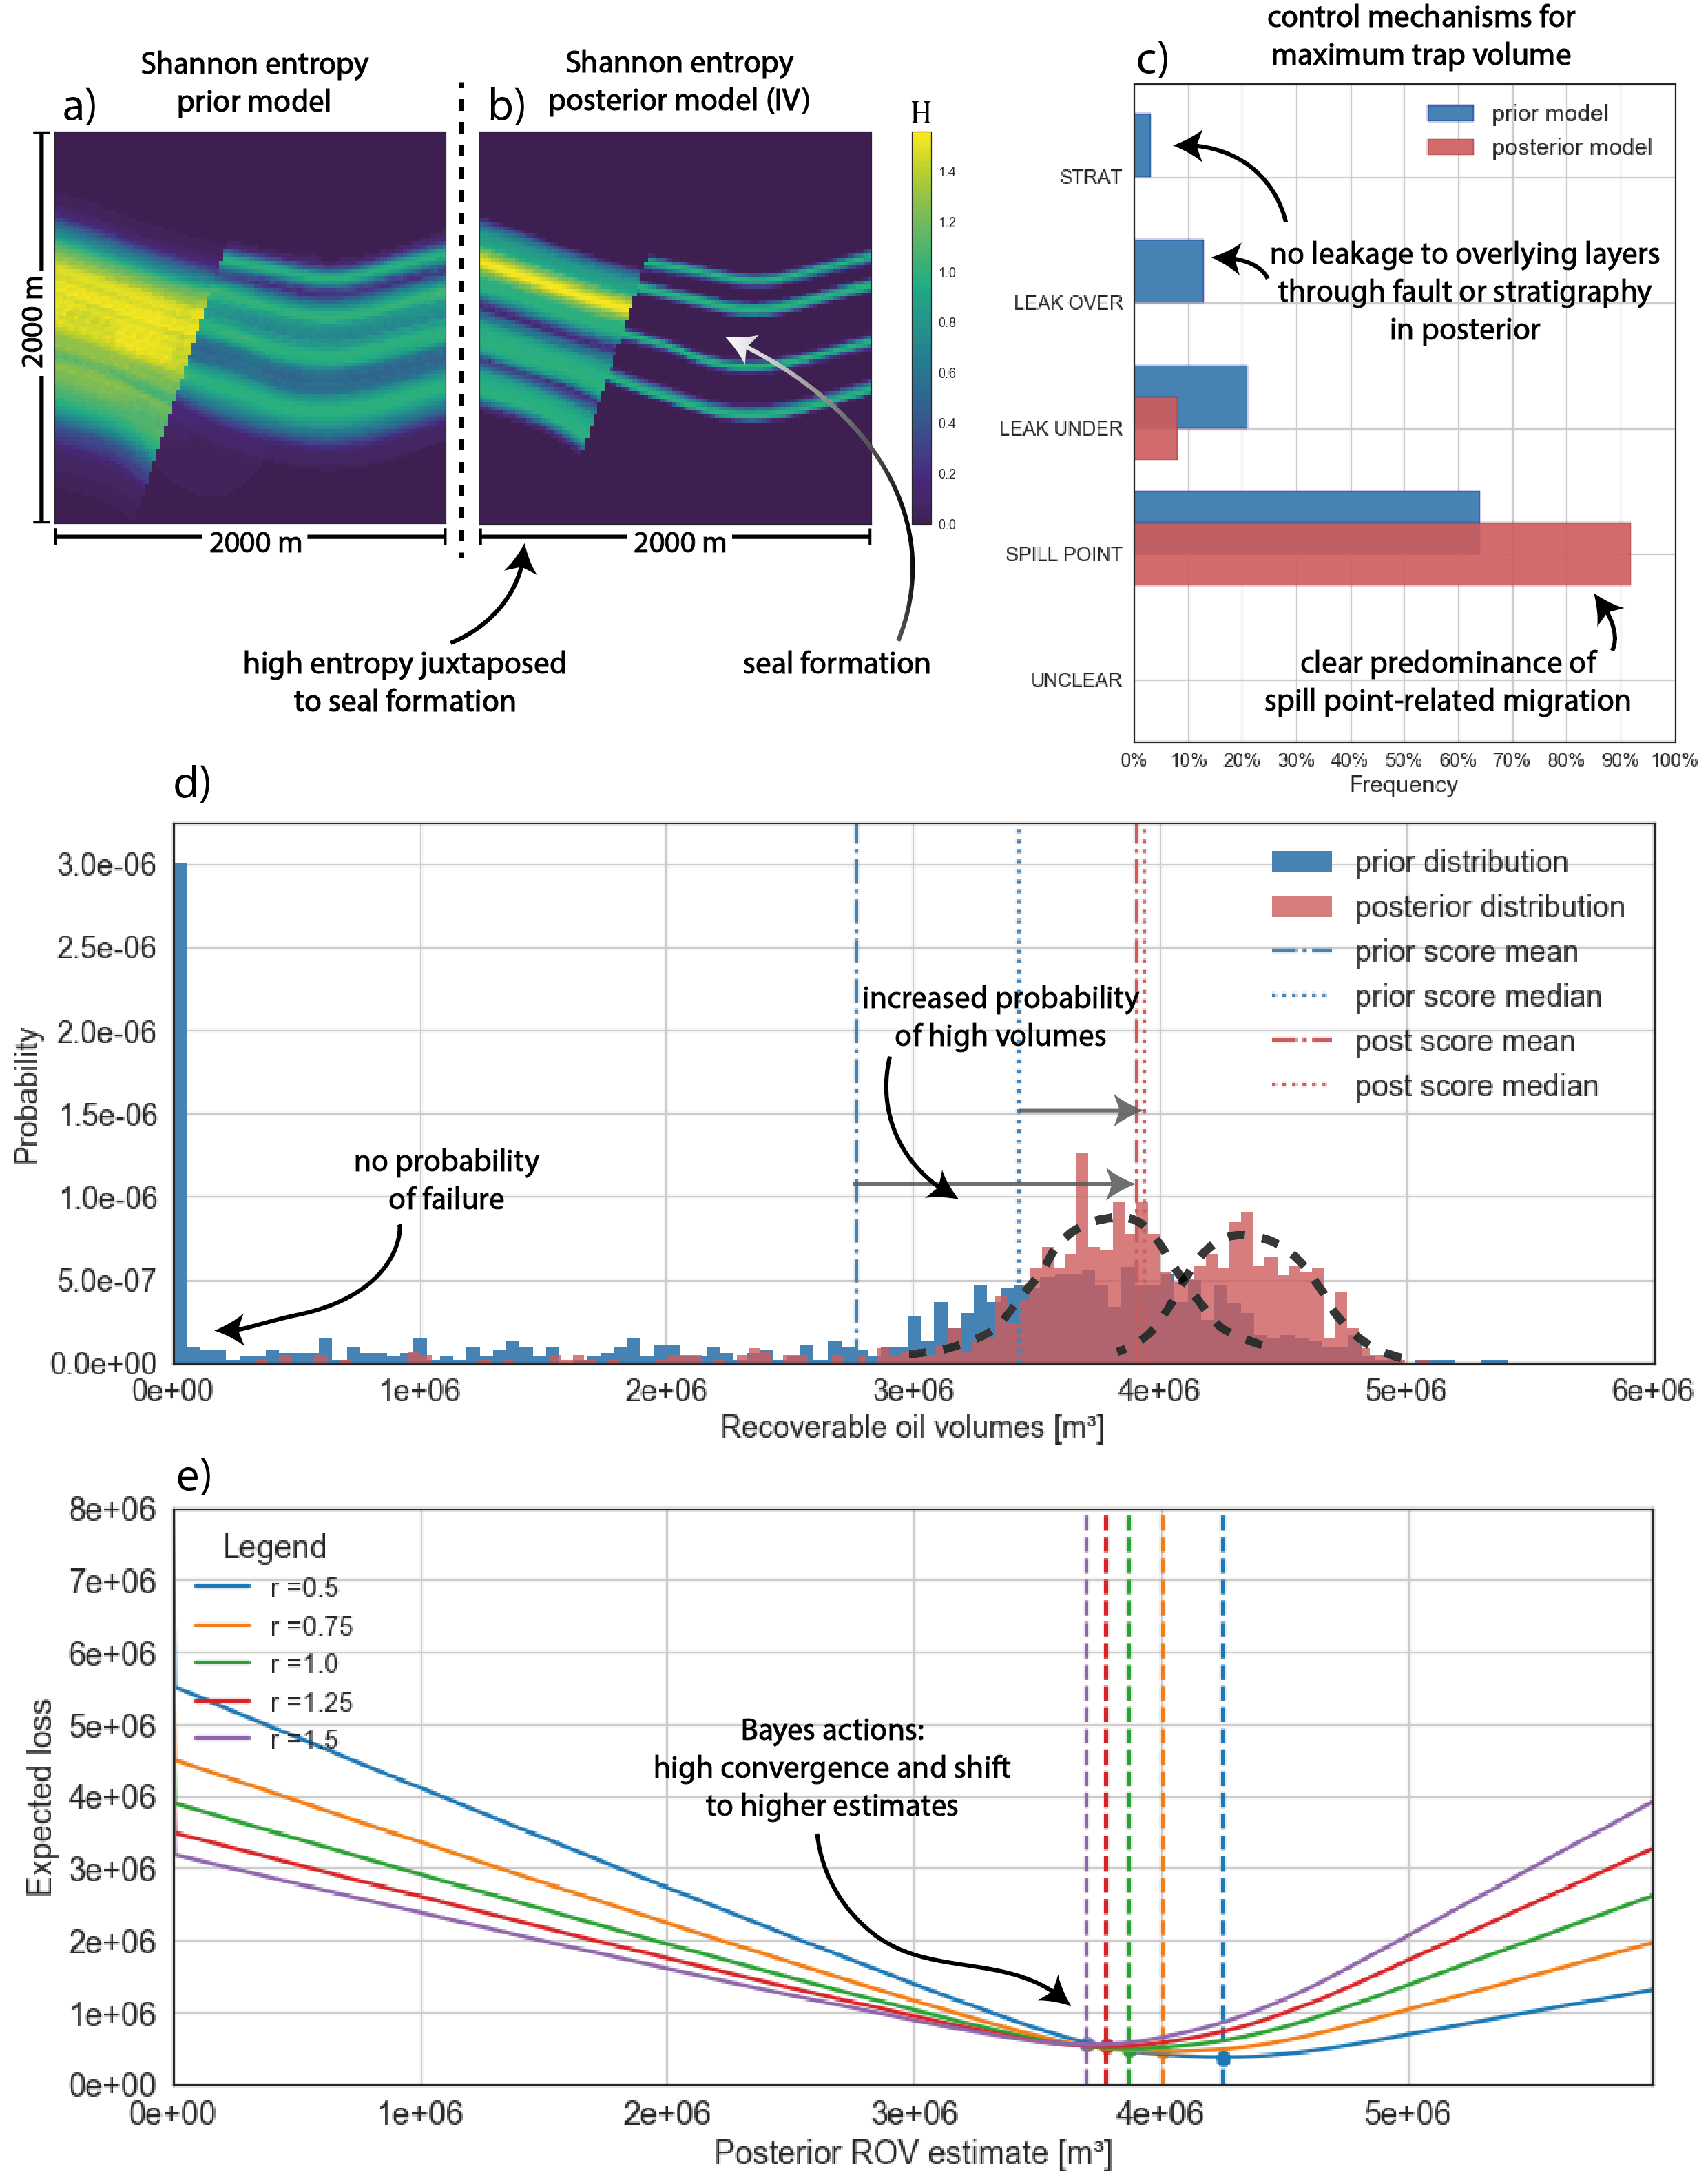
\includegraphics[width=1\textwidth]{figures/ML4}
%				\caption{....}
%				\label{fig:ML4}
%			\end{minipage}
%			\hspace{\fill}
%			\begin{minipage}[t]{0.32\textwidth}
%				\centering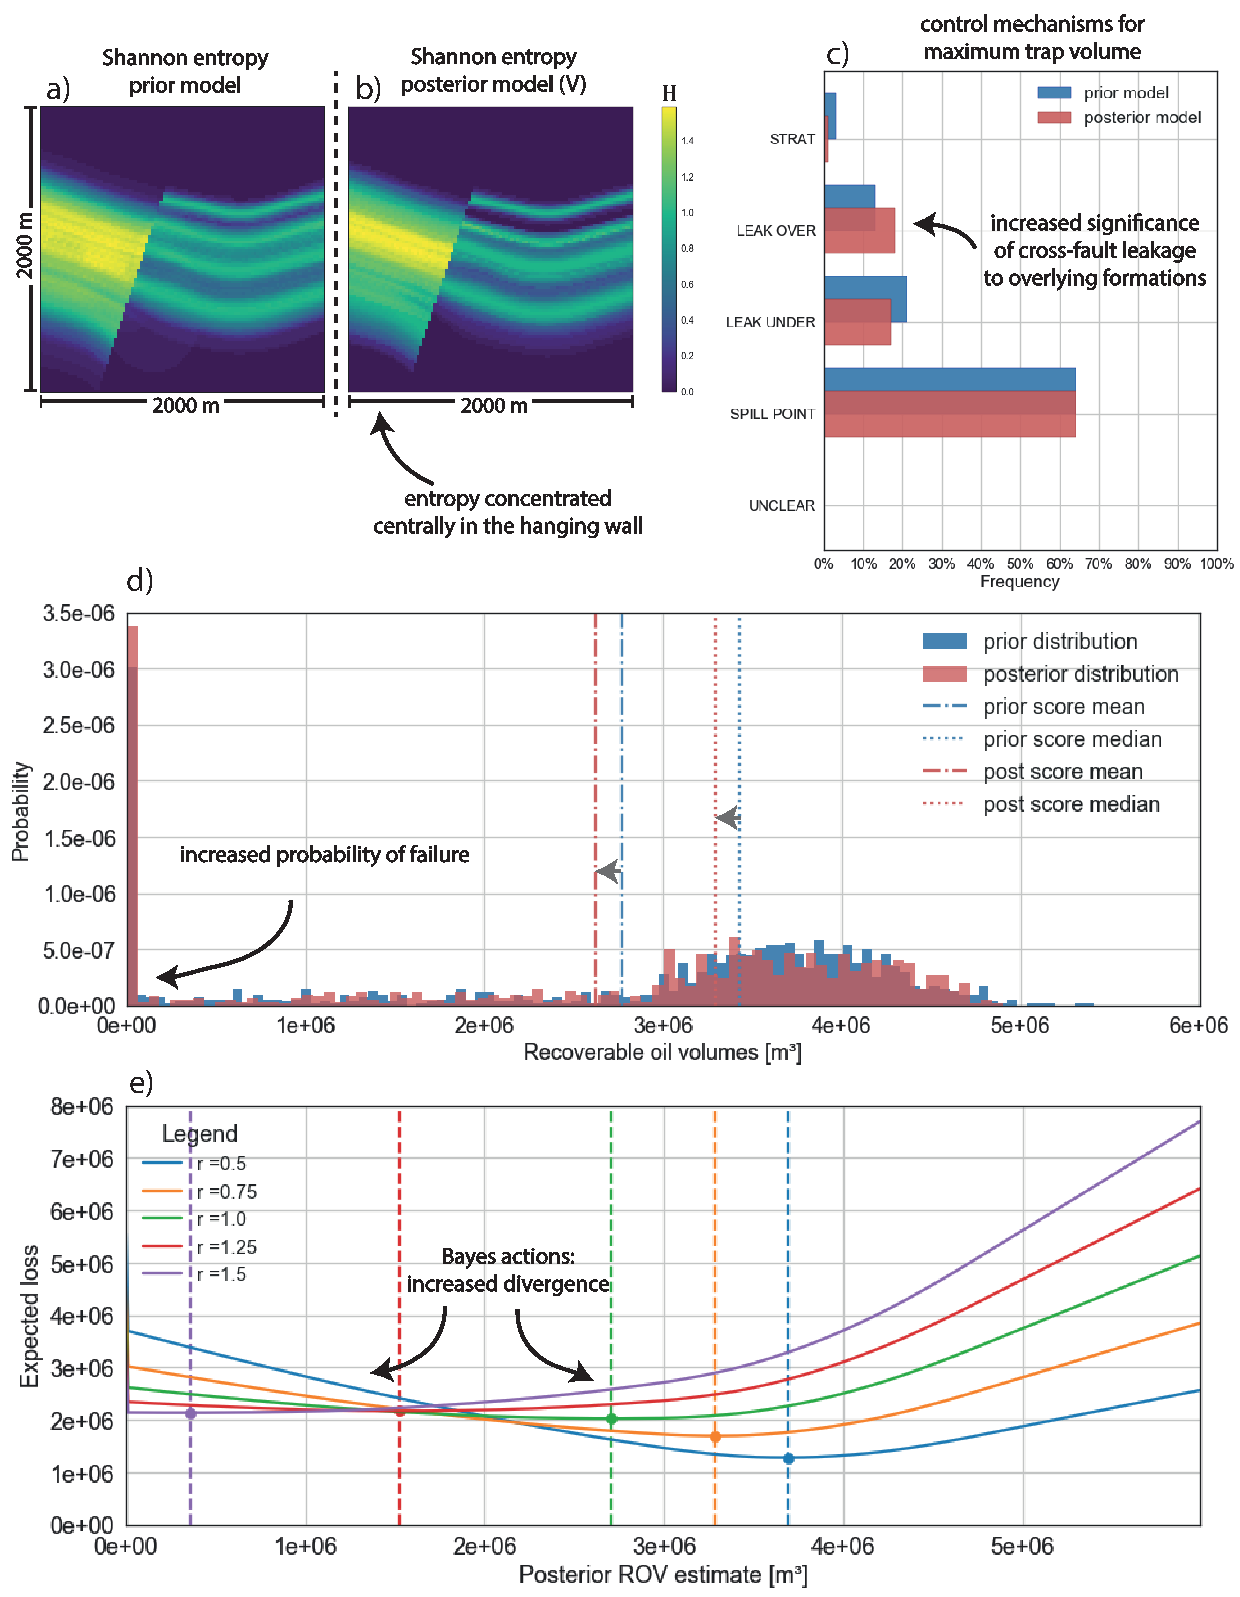
\includegraphics[width=1\textwidth]{figures/ML5}
%				\caption{...}
%				\label{fig:ML5}
%			\end{minipage}	
%		\end{minipage}
%	\end{figure}
%	\vspace{0.2em}



	%\begin{figure}
	%	\begin{minipage}{.94\textwidth}
	%		\centering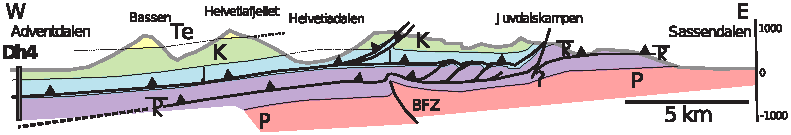
\includegraphics[width=\textwidth]{figures/cross_section}
	%		\caption{...}
	%		\label{fig:cross_section}
	%	\end{minipage}
	%\end{figure}
	%\vspace{0.2em}
	%\vfill

\end{myblock}				

		}\end{minipage}\end{beamercolorbox}
	\end{column}
	
	\begin{column}{.249\textwidth}
		\begin{beamercolorbox}[center]{postercolumn}
			\begin{minipage}{.98\textwidth}  % tweaks the width, makes a new \textwidth
				\parbox[t][\columnheight]{\textwidth}{ % must be some better way to set the the height, width and textwidth simultaneously	

\begin{myblock}{3 - Results (continued)}
Posterior ROV probability distributions are realized depending on the nature of likelihoods implemented in the Bayesian inference step. Applying the custom loss function shows that the various Bayes actions shift according to the characteristics of this underlying	value distribution. While bimodality and overall uncertainty lead to separation, risk-averse and risk-friendly decisions converge and decrease in expected loss given narrower unimodal distributions. A decisive factor in our model is seal reliability, as it defines the probability of complete trap failure. Two examples are summarized in Figures \ref{fig:ML4} and \ref{fig:ML5}.
\end{myblock}
		
\begin{myblock}{4 - Conclusions}
%\vspace{0.5em}
%								\begin{figure}
%									\begin{minipage}{0.8\textwidth}
%									\centering
%									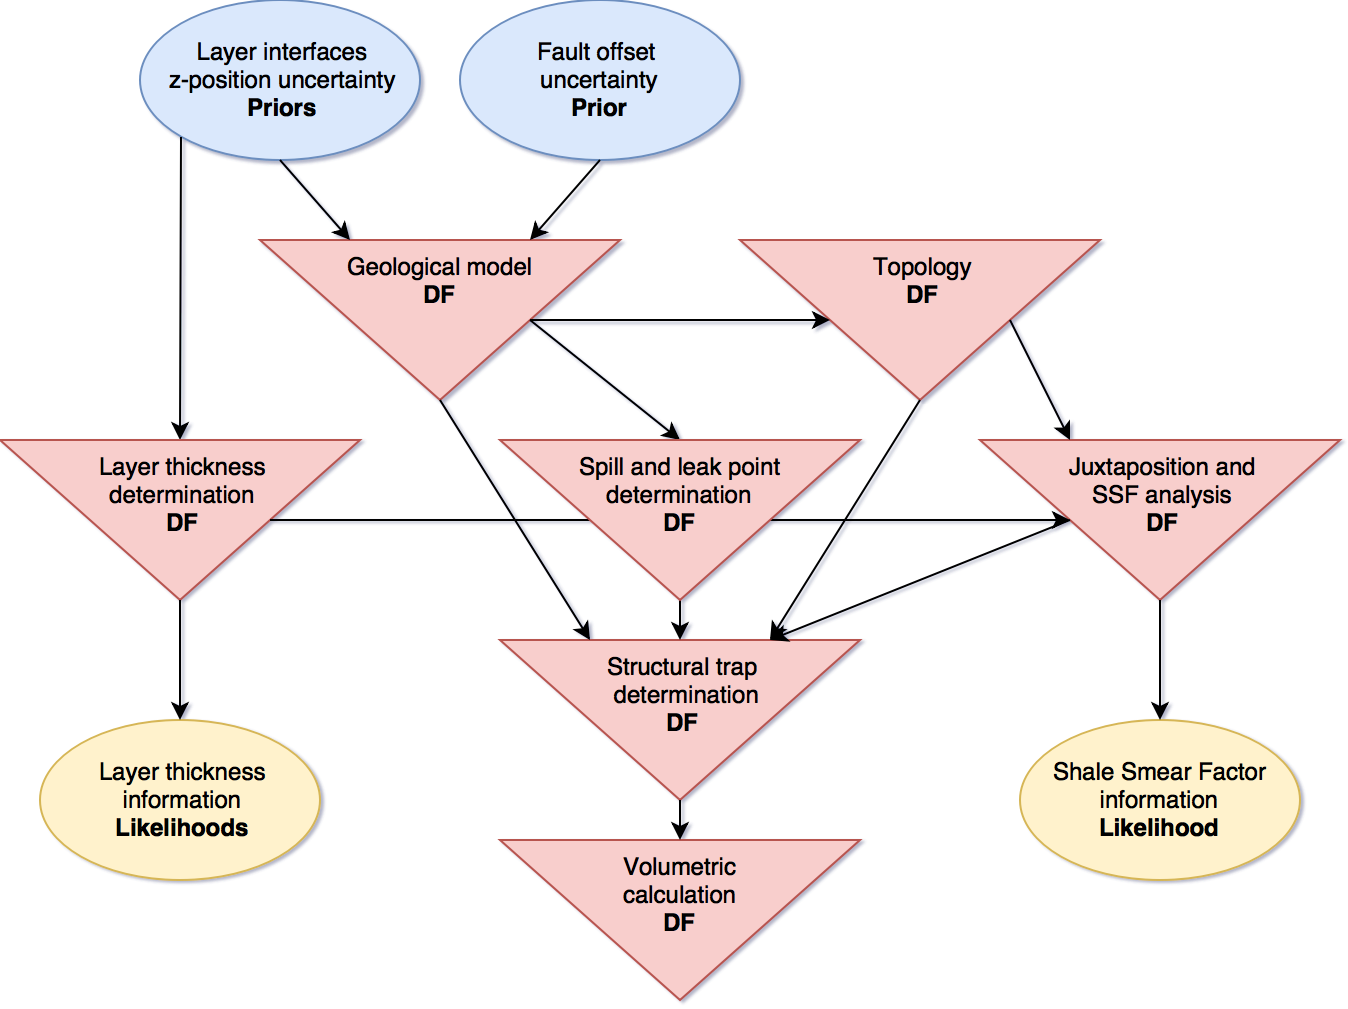
\includegraphics[width=1\textwidth]{figures/model_network}
%									\caption{Illustration of the probabilistic model as a hierarchical Bayesian network after \citet{koller2009probabilistic}. Stochastic nodes are represented by ellipses (blue for
%									priors, yellow for likelihoods). Deterministic functions are depicted as triangles in
%									red. Arrows indicate direct connections from parent to child nodes.}
%									\label{fig:model_network}
%									\end{minipage}
%								\end{figure}

\begin{itemize}
\item The degree of \textbf{decision convergence} can be considered a measure for the state of knowledge and its inherent uncertainty at the moment of decision making.
\item This decisive uncertainty does not change in alignment with model uncertainty but depends on alterations of \textbf{critical parameters} and respective interdependencies.
\item Actors are \textbf{affected differently} by one set of information, depending on their risk affinity.
\item It is important to \textbf{identify the model parameters} which are most influential for the final decision in order to
\textbf{optimize the decision-making process}.
\end{itemize}
These results and conclusions refer to a generic hydrocarbon system case study but are transferable to other fields where decisions
are based on uncertain geological models, for example in hydrogeological or geothermal exploration.
%\vspace{0.3em}
%\begin{figure}
%	\begin{minipage}{0.95\textwidth}
%		\begin{minipage}[t]{0.36\textwidth}
%			\vspace{0pt}
%			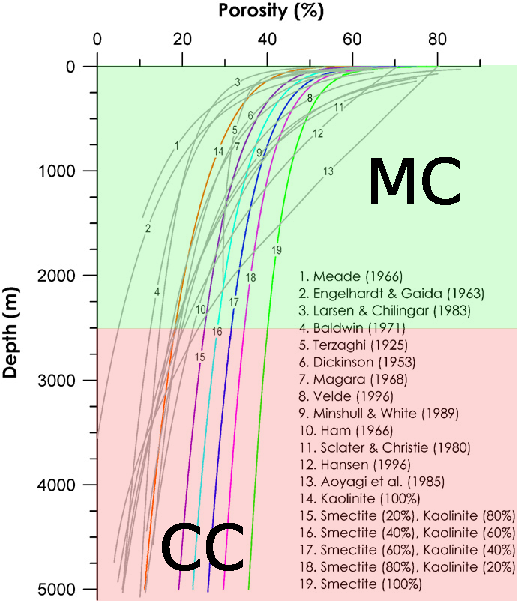
\includegraphics[width=\textwidth]{figures/compaction.pdf}
%		\end{minipage}\hfill
%		\begin{minipage}[t]{0.22\textwidth}
%			\vspace{0pt}
%			\caption{
%			Comparison of porosity–depth trend studies and experimental results for shales and
%argillaceous sediments. While for E\&P projects the seal integrity is proven by the abundance of hydrocarbons, for \ce{CO2} storage it remains uncertain. Controlling factors are clay mineral and pore fluid composition, grain sizes, pore pressure and the influence of mechanical \textbf{(MC)} and chemical compaction \textbf{(CC)}. Because core sampling of seal layers is expensive, experimental studies and global databases might be auxiliary. Still, extrapolation of experimental results has limited validity for natural anisotropy and the influence of chemical compaction \citep{mondol_experimental_2007}.
%			} \label{fig:compaction}
%		\end{minipage}\hfill
%		\begin{minipage}[t]{0.38\textwidth}
%			\vspace{0pt}
%			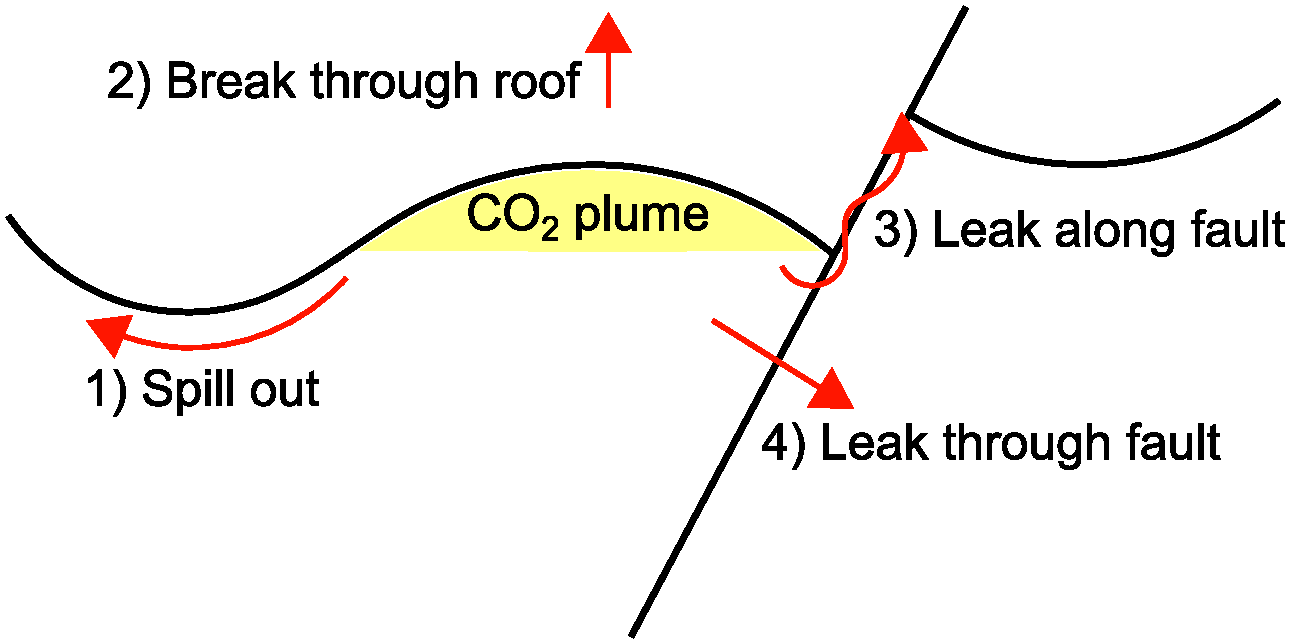
\includegraphics[width=\textwidth]{figures/leakage.pdf}
%			\caption{
%			Different leakage scenarios for a \ce{CO2} storage project which are subject to uncertainty. To prevent a spill out of the storage formation \textbf{(1)}, the storage capacity must be estimated. A break of \ce{CO2} through the formation's roof \textbf{(2)} depends on seal properties and knowledge of fracture pressures (see figure \ref{fig:compaction}). Evaluation of leakage along \textbf{(3)} or through \textbf{(4)} a fault requires the analysis of juxtaposition and smearing. Sub-seismic faults represent an additional risk. Still, the highest risk of leakage exists in close proximity to wells (Figure based on lecture notes, lecture by K. Indrevær \& A. Braathen, 15.6.2017).
%			} \label{fig:leakage}
%		\end{minipage}
%	\end{minipage}
%\end{figure}
	


\end{myblock}			
								
					
\begin{myblock}{5 - References}
	\footnotesize
	\bibliography{./references}
\end{myblock}

\begin{myblock}{6 - Further information}
\small
Geological models were created in a Python environment using GemPy \citep{gmd-2018-61} and integrated into a probabilistic framework via PyMC \citep{salvatier2016pymc3}. 

This research poster is based on a master thesis submitted to the Institute of Computational Geoscience and Reservoir Engineering (CGRE) at the RWTH Aachen University in 2017 (see \citet{stamm2017}).
		
		%\begin{minipage}[t]{0.72\textwidth}	
		%\textbf{Contact:}
		%	\begin{itemize}
		%	\item E-mail: fabian.stamm@rwth-aachen.de
			%\item Phone: + 49 174 5231499
		%	\end{itemize}

			
		%\end{minipage}\hfill
		%\begin{minipage}[t]{0.23\textwidth}
		%	\vspace{0em}
		%	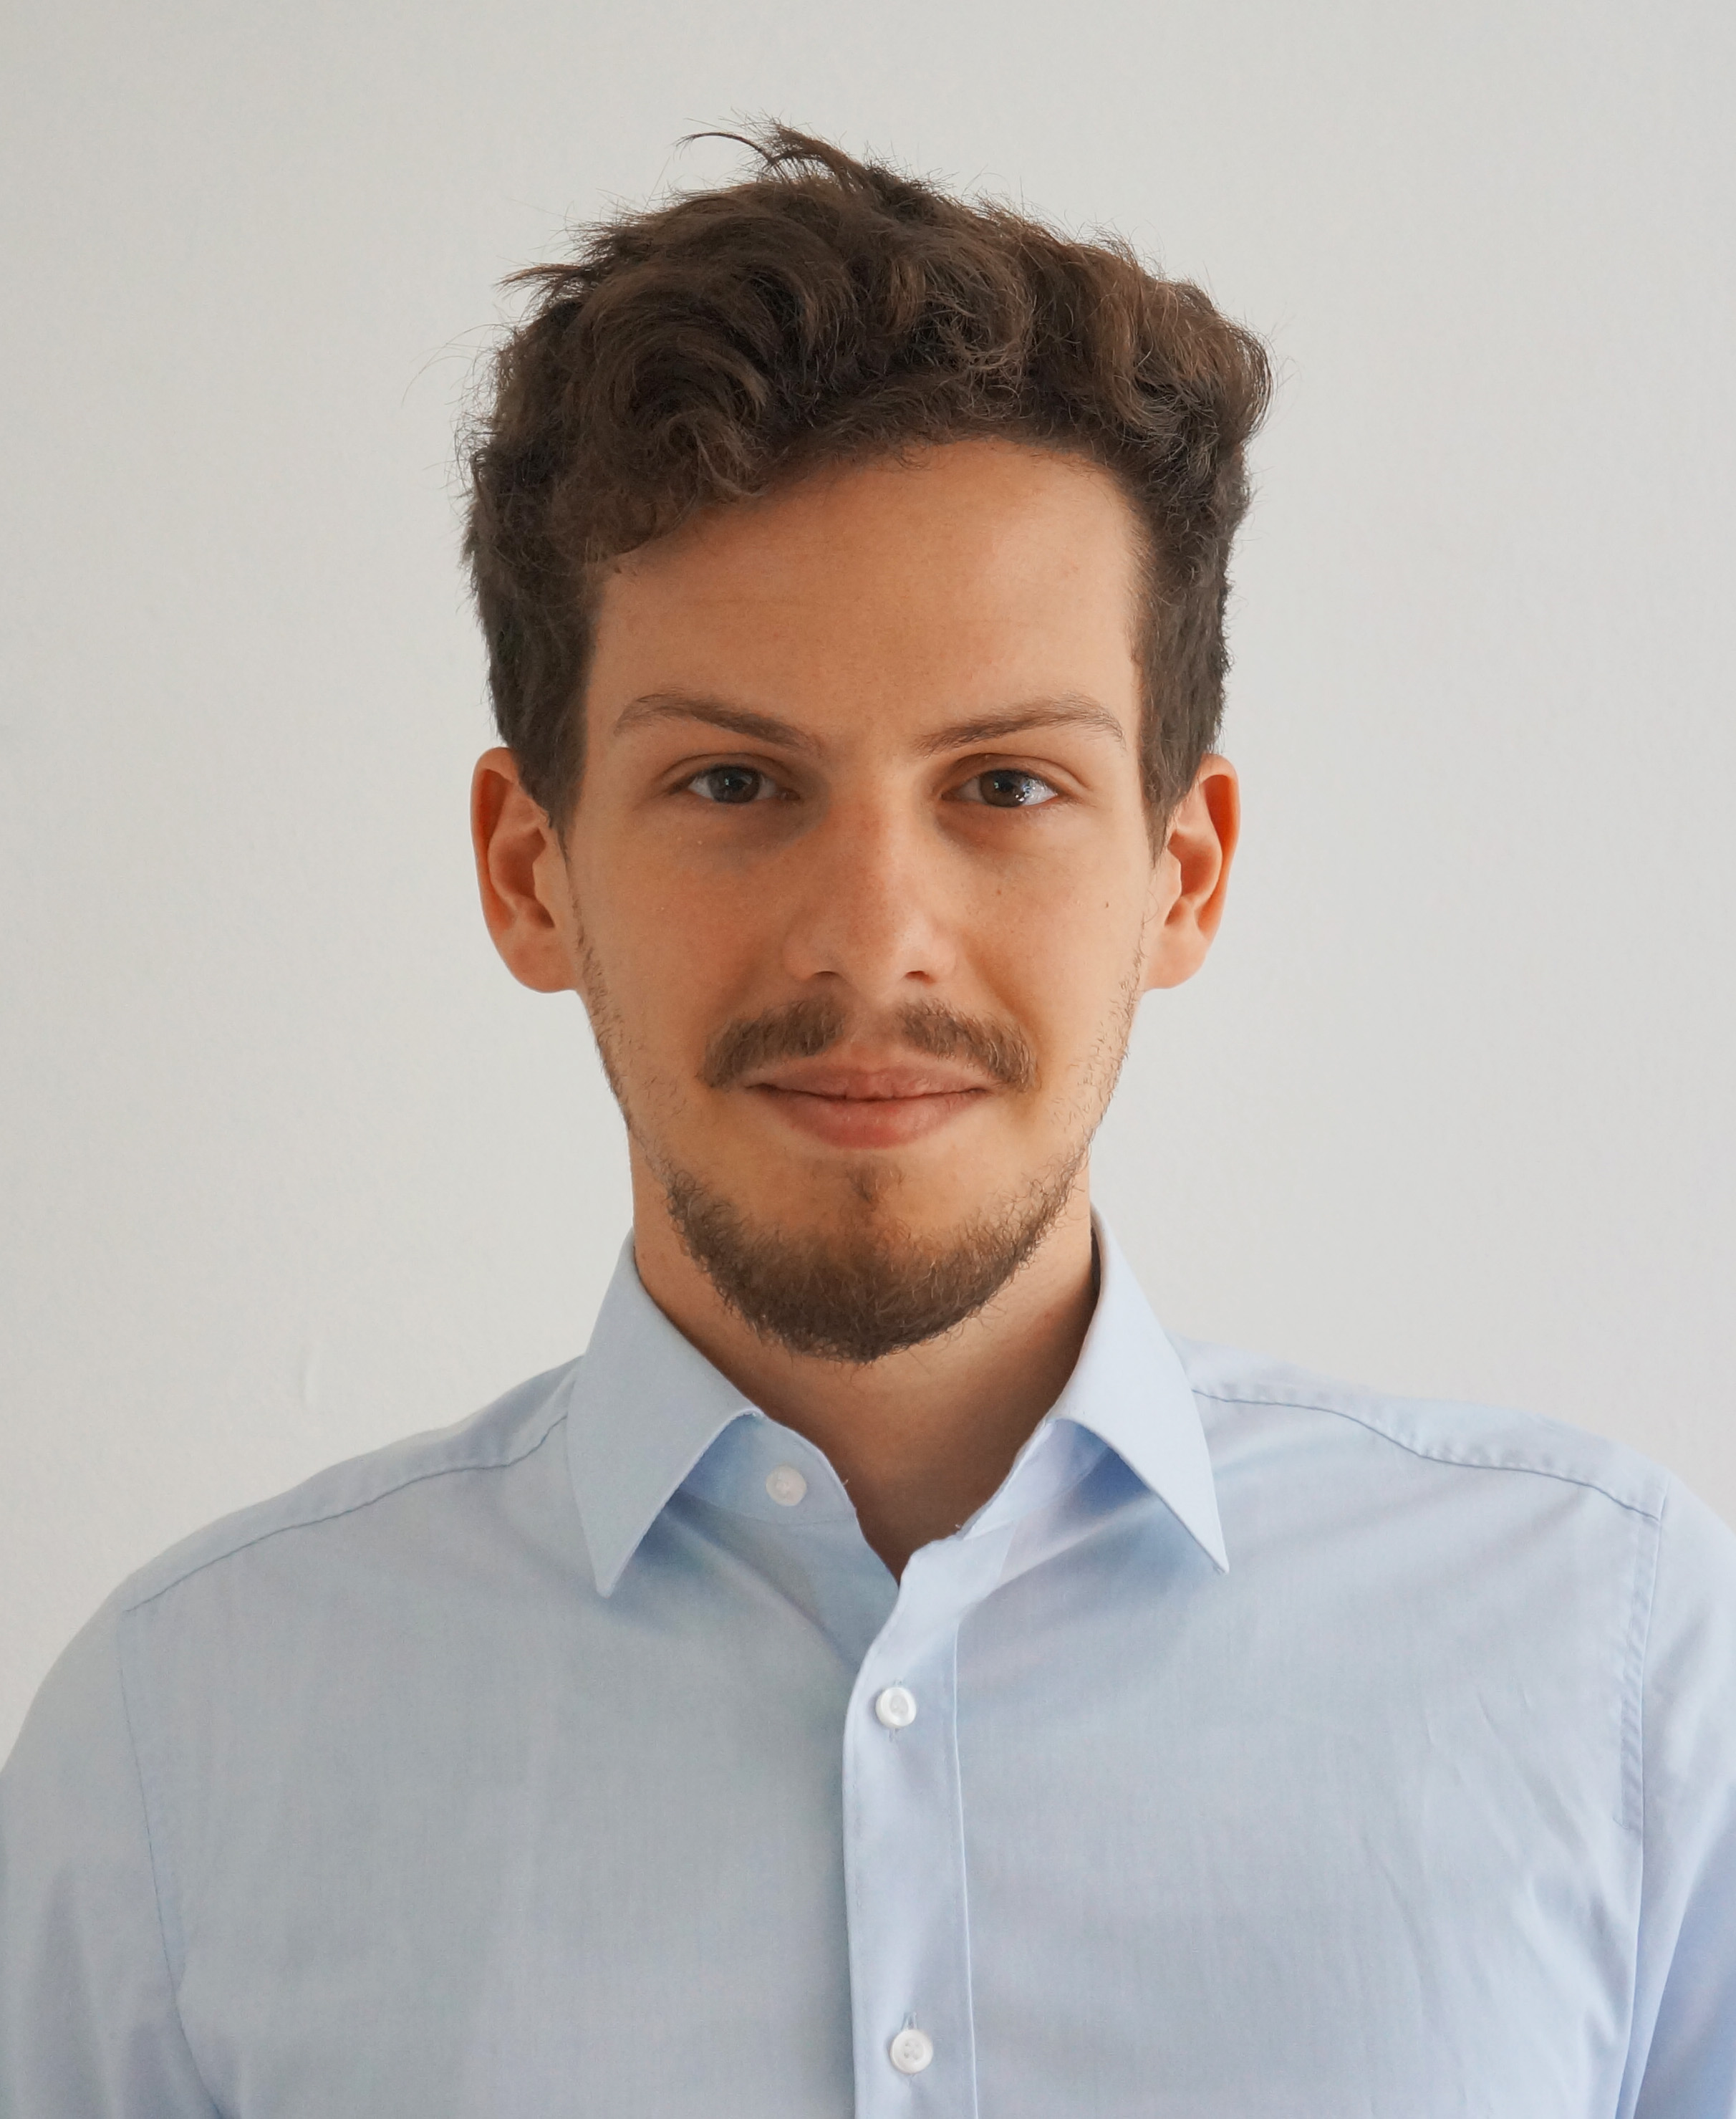
\includegraphics[width=1\textwidth]{figures/author}
		%	\vspace{0.5em}
		%\end{minipage}
		
			%\vspace{0.4em}
			%\vfill



\end{myblock}\vfill		
				
	}\end{minipage}\end{beamercolorbox}
		\end{column}
		
\end{columns}
\end{frame}
\end{document}
